\documentclass[11pt]{article}
\usepackage[utf8]{inputenc}
\usepackage[T1]{fontenc}
\usepackage{amsmath}
\usepackage{amsfonts}
\usepackage{amssymb}
\usepackage[version=4]{mhchem}
\usepackage{stmaryrd}
\usepackage{hyperref}
\hypersetup{colorlinks=true, linkcolor=blue, filecolor=magenta, urlcolor=cyan,}
\urlstyle{same}
\usepackage{multirow}
\usepackage{graphicx}
\usepackage[export]{adjustbox}
\graphicspath{ {./images/} }

\begin{document}
Venture Debt

Venture debt is any form of debt financing provided to venture capital-backed companies. They are usually accompanied by a venture capital equity round. Companies typically use venture debt to reduce equity dilution and to have a larger cash reserve to reach their next valuation target. Given the higher risk of venture debt, investors earn high interest rates as well as warrants for participating in the increase in the equity value of the firm.

\section*{Overview of Venture Debt}
Startups are generally not creditworthy enterprises. They have few or no assets and little cash flow, thus they cannot access debt from traditional lenders. Equity is typically the way to finance startups. The failure rate for startups is high, with estimates that over $90 \%$ of new startups fail, ${ }^{1}$ Max Marmer et al. (2011), Startup Genome Report On Premature Scaling. In Startup Genome Report. \href{https://innovationfootprints.com/wp-content/}{https://innovationfootprints.com/wp-content/} uploads/2015/07/startup-genome-report-extra-onpremature-scaling.pdf while another report estimates that $75 \%$ of venture capital (VC)-backed startups fail. ${ }^{2}$ Wall Street Journal (2012), The Venture Capital Secret: 3 out of 4 Start-ups Fail. \href{https://www.wsj.com/articles/}{https://www.wsj.com/articles/} SB10000872396390443720204578004980476429190 The differences between VC-backed companies and nonVC-backed companies is further emphasized when considering the failure rate, acquisition rate, and initial public offering (IPO) rate. Using over 20 years of data that tracks US business establishments, Puri and Zarutskie (2011) ${ }^{3}$ Puri, Manju, and Rebecca Zarutskie (2011), On the Lifecycle Dynamics of Venture-Capital- and NonVenture-Capital-Financed Firms. National Bureau of Economic Research. \href{https://www.nber.org/system/}{https://www.nber.org/system/} files/working\_papers/w14250/w14250.pdf found that VCbacked companies have lower failure rates, higher acquisition rates, and higher IPO rates than non-VC-backed companies:

\begin{itemize}
  \item The cumulative failure rate of VC-backed companies by the end of year five is only $19 \%$, while for non-VC-backed companies it is $51 \%$.
  \item The cumulative acquisition rate of VC-backed companies by end of year five is $4.1 \%$, while for non-VC-backed companies it is $0.36 \%$.
  \item The cumulative IPO rate of VC-backed companies by end of year five is $7.58 \%$, while for non-VC-backed companies it is $0.02 \%$
\end{itemize}

Despite the high risk associated with startups, there is a large and growing market for startup lending, called venture debt. A venture lender provides the debt financing over a term of two to four years, which includes an equity kicker for the lender to purchase stock, preferred stock, or both. Unlike traditional loans, venture debt typically does not require any collateral or positive cash flows from the startup.

Venture lenders can be categorized into two main groups. The first group is the specialized banks. Unlike the commercial banks, which do not offer venture debt, specialized banks work with startups and offer venture debt as a core offering. The second group is venture debt funds. According to Rassenfosse and Fischer (2016), ${ }^{4}$ de Rassenfosse, G., and T. Fischer (2016), Venture Debt Financing: Determinants of the Lending Decision. Strategic Entrepreneurship Journal 10(3): 235-256. \href{https://papers.ssrn.com/sol3/papers.cfm?abstract}{https://papers.ssrn.com/sol3/papers.cfm?abstract} id=1909602 venture lenders can overcome the barriers of lending to non-creditworthy and informationally opaque startups because of two key conditions:

\begin{itemize}
  \item Venture capital backing substitutes for a startup's positive cash flow.
  \item There is preference for startups that offered warrants.
\end{itemize}

This highlights the important aspect of the business model of venture debt lenders. Venture debt follows venture capital, and it is usually raised after the startup has obtained venture capital, not before. Sometimes venture debt is raised alongside venture capital. This is notable because the lenders are not lending on the creditworthiness of the startups, but they are lending on the creditworthiness of the venture capital firm or syndicate for the follow-on round of financing where venture lenders will be repaid.

Venture lenders will also request warrants to purchase company stock in an amount typically calculated as a percentage of the loan amount. The warrants are to compensate for the higher risk of loan default. The warrant coverage ranges from $5 \%$ to $15 \%{ }^{5}$ Tom Taulli (2008), How Venture Debt Financing Works and How to Get It, In Business Week Sept. 19, 2008. Extracted from: \href{https://www.bloomberg.com/news/articles/2008-09-19/how-venture-debt-financing-works-and-how-to-getitbusinessweek-business-news-stock-market-}{https://www.bloomberg.com/news/articles/2008-09-19/how-venture-debt-financing-works-and-how-to-getitbusinessweek-business-news-stock-market-} and-financial-advice of the value of the loan, and are often vested at the time of loan funding. The warrants give the venture lender the right to buy shares in the future at the per-share price of the most recent equity funding round. The resulting dilution is typically less than $2 \%$ of equity.

\begin{center}
\begin{tabular}{|c|c|c|c|}
\hline
Category & Funds & Banks & \begin{tabular}{l}
International financial \\
Institutions (IFIs) \\
\end{tabular} \\
\hline
\begin{tabular}{l}
Relationship \\
duration \\
\end{tabular} & - Usually 2-5 years of investment & \begin{tabular}{l}
- Long term view, future corporate client \\
pipeline \\
\end{tabular} & - Long term view \\
\hline
Pricing & \begin{tabular}{l}
- Typically more expensive, dictated by \\
hurdle rates agreed with LPs of the fund \\
\end{tabular} & - Typically cheaper, balance sheet funding & - Typically cheaper, balance sheet funding \\
\hline
\begin{tabular}{l}
Ancillary business \\
required \\
\end{tabular} & - No & - Yes (e.g. deposits, credit cards, FX) & - No \\
\hline
Warrants & \begin{tabular}{l}
- Typical for early stage venture debt \\
- Higher probability to be exercised \\
\end{tabular} & \begin{tabular}{l}
- Typical for early-stage venture debt \\
- Higher probability to be sold back \\
\end{tabular} & - Usually not applicable \\
\hline
\begin{tabular}{l}
Business \\
characteristics \\
\end{tabular} & - High growth businesses & - High growth businesses & \begin{tabular}{l}
- Innovative, socially beneficial and \\
responsible businesses \\
\end{tabular} \\
\hline
\multirow[t]{2}{*}{Geographic focus} & - Demand and profit driven & - Demand and profit driven & \begin{tabular}{l}
- Social objectives of equal access to \\
capital to boost the economy \\
\end{tabular} \\
\hline
 & Funds & Banks & IFIs \\
\hline
Examples & \begin{tabular}{l}
Boost \& Co. \\
: Bootstrap Europe \\
Harbert European Growth Capital \\
Kreos Capital \\
\end{tabular} & \begin{tabular}{l}
Barclays \\
: Goldman Sachs \\
Silicon Valley Bank \\
\end{tabular} & \begin{tabular}{l}
. European Investment Bank \\
- KFW Bank \\
\end{tabular} \\
\hline
\end{tabular}
\end{center}

\section*{Main Categories of Venture Lenders}
Source:Venture Debt in Europe Market Overview provided by Deloitte for the European Investment Bank. Data from Venture debt providers' websites.

Given that it is a nascent market, there are no official data and statistics on the size of the venture debt market. However, there are estimates that peg venture debt to $10 \%-15 \%$ of the value of venture capital invested. According to Pitchbook, venture debt is more commonplace in the United States, accounting for $78 \%$ of global venture debt deal count. This is a function of the scale of VC funding and prevalence of non-bank funding in the United States. According to National Venture Capital Association, as of the end of 2019, about US\$130 billion is deployed into startups in the US venture market. This puts the US venture debt market around $\$ 10-12$ billion. Europe is the next largest venture debt market, accounting for $10 \%$ of global venture debt deal count. European venture debt shows a similar pattern to European VC, with concentrations in the UK, France, and Germany. Lastly, venture debt is still relatively small in other regions, which account for only $6 \%$ of global venture debt deal count. In India and Southeast Asia, venture debt deal size ranges from US\$1 million to US\$2 million. The small deal size makes it less attractive for abank.

\section*{Typical Terms of Venture Debt}
Venture lenders typically target a 12-18\% IRR for each transaction. ${ }^{6}$ Winston \& Strawn, BVCA (2010), The Rise of Venture Debt in Europe.

\href{https://www.bvca.co.uk/Portals/o/library/Files/News/2010/2010_0053_venture_debt_report_may.pdf}{https://www.bvca.co.uk/Portals/o/library/Files/News/2010/2010\_0053\_venture\_debt\_report\_may.pdf}? ver=2012-05-02-162120-000 The IRR can be broken down into three components:

\begin{enumerate}
  \item Fee income, which could make up around $1-2 \%$ of capital

  \item Interest income which could make up around $9 \%$ to $15 \%$ yield on capital

  \item Warrant gains, which act as a kicker for the return

\end{enumerate}

Venture debt terms are often contextual. Loan types and sizes may vary significantly, based on the scale of the startup, the quantity and quality of venture capital raised to date, and the objective for which the venture debt is raised. The amount of venture debt available is linked to the amount of venture capital the startup has raised. Loan sizes tend to vary between $20 \%$ and $35 \%^{7}$ Shane Anderson (2018), The Role of Venture Debt in Booming Tech Market, Silicon Valley Bank website. \href{https://www.svb.com/blogs/shane-anderson/the-role-of-venture-debt-in-a-booming-tech-market}{https://www.svb.com/blogs/shane-anderson/the-role-of-venture-debt-in-a-booming-tech-market} of the amount raised in the most recent equity round. Other typical terms are shown in the exhibit below.

Key Terms of Venture Debt

\begin{center}
\begin{tabular}{|c|c|}
\hline
Category & Venture Debt \\
\hline
Business characteristics & Medium to late venture-backed startup experiencing high growth \\
\hline
Ticket Size & US\$1 million to US\$20 million \\
\hline
Tenor & 1 to 3 years \\
\hline
\begin{tabular}{l}
Interest Rate (excluding \\
warrants) \\
\end{tabular} & $9 \%$ to $15 \%$ \\
\hline
Fees & Arrangement Fees, Prepayment Fees, Backend/Success Fees \\
\hline
Dilution & \begin{tabular}{l}
- Warrant coverage of typically $5 \%$ to $15 \%$ of loan amount \\
- Generally, a small fraction of equity; $<2 \%$ due to warrants \\
\end{tabular} \\
\hline
Financial Covenant & None \\
\hline
Industry Focus & All sectors, with focus on technology and healthcare \\
\hline
Repayment Schedule & \begin{tabular}{l}
- Often includes an interest-only period, followed by scheduled amortization. Some loans may be interest-only with $100 \%$ of \\
principal due at final maturity. \\
- Typically repaid at the next equity founding round \\
\end{tabular} \\
\hline
\end{tabular}
\end{center}

Source: CAIA Association. Data from various venture debt providers' websites and market research.

\section*{The Demand for Venture Debt}
Venture debt can be attractive for startups that seek additional funds to grow without raising additional equity. There are four key reasons why a startup would raise venture debt in addition to venture capital:

\begin{enumerate}
  \item Reduce equity dilution. Venture debt allows startups to raise capital with lower dilution than raising a similar amount of venture capital. This allows founders to reduce their shareholding dilution from venture capital and maintain higher stake and control of their company.

  \item Debt financing is cheaper than equity. Assuming strong growth of the startup, adding leverage will increase returns for the founders and existing VC investors. In addition, the interest paid for venture debt is also tax deductible for the profitable startup.

  \item Flexible structure. Raising venture debt is generally quicker than VC fundraising, which requires establishment of a new valuation and may introduce valuation problems. In addition, it requires less management focus. Furthermore, venture lenders do not have board seat or voting rights in the company.

  \item Additional capital to achieve valuation milestones and make the company more valuable. Venture debt has the potential to delay equity financing in anticipation of higher valuation through achieving the next milestone or valuation driver. This could reduce the number of rounds of equity financing needed and thereby substantially reduce dilution for founders.

\end{enumerate}

\section*{The Risks and Reward of Venture Debt}
Venture debt has a different risk and return profile than Venture Capital (VC). Lenders are naturally risk averse. Their returns depend on having their loan repaid with interest and few defaults. Venture lenders are no different. On the other hand, VC can afford to have some of their startups fail because of the outsized returns from those startups that succeed. For venture lenders, it may seem like they are taking equity risk by providing capital to risky startups, but they only obtain debt like returns with some equity kicker from the warrants if the startup is successful. The type of binary outcomes in venture investing can adversely impact a venture lender because they cannot achieve the type of 10x returns that VC can sometimes obtain; the best outcome a venture lender can achieve are singles and doubles and they are not sufficient to make up for large capital losses in some startups. The exhibit below illustrates the relative return performance between VC and venture debt under different scenarios. For the venture lender, ensuring low loss rates is still more important than the potential upside that the warrants can provide.

\begin{center}
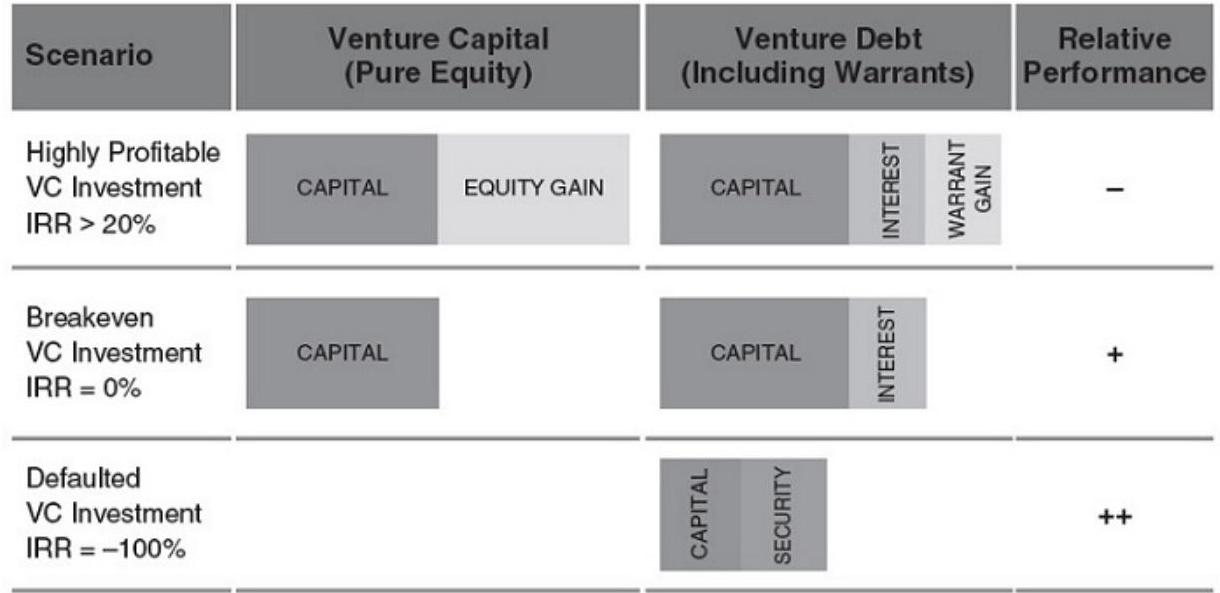
\includegraphics[max width=\textwidth]{2024_04_10_cdc3d7c1e12c48419e6bg-5}
\end{center}

\section*{Comparing the Return Profiles of VC and Venture Debt}
Source: The British Private Equity and Venture Capital Association (BVCA), The Rise of Venture Debt in Europe. Report Sponsored by Winston \& Strawn. \href{https://www.bvca.co.uk/Portals/0/library/Files/News/2010/2010_0053_venture_debt_report_may.pdf?ver.2012-05-02-162120-000}{https://www.bvca.co.uk/Portals/0/library/Files/News/2010/2010\_0053\_venture\_debt\_report\_may.pdf?ver.2012-05-02-162120-000}

Even though venture lenders are essentially lending to cash-burning VC-backed startups with no track records, tangible assets, or personal guarantee from founders, the reality is that venture loans have achieved remarkable low loss rates on invested capital. According to Uribe and Mann (2017), ${ }^{8}$ González-Uribe, Juanita, and William Mann (2017), New evidence on venture loans. SSRN Working Papers. \href{https://www.dropbox.com/s/519xntjdzrs1xbg/LBS}{https://www.dropbox.com/s/519xntjdzrs1xbg/LBS} PE symposium.pdf their review of several venture lender's portfolio showed that the loss rate of about $3 \%$, which is surprisingly low when one considers the failure rate of venture-backed startups. The low loss rate is because venture-backed startups do not typically fail in the early rounds, only after the venture debt has been repaid. Therefore, startup failures far outnumber loan defaults. When a VC makes an initial investment at the early stage, it is almost certain that the VC will make or attract a follow-on investment. In addition, VCs do not want to earn the reputation in the startup community of not supporting their portfolio companies, thus they often reserve capital for follow-on investments in their portfolio companies. Hence, venture lenders have a different exit strategy than VCs; they just need to provide funding until the subsequent round of equity financing.

There are differences in the reward and motivation between bank and non-bank venture lenders. A typical venture loan ranges from US\$1 million to US\$20 million. A bank venture lender or their affiliated entities typically provide venture debt at the lower end of the range. They are also able to offer lower interest rates compared to non-bank venture lenders. The key motivation for bank venture lenders is the opportunity to secure the startup's deposit accounts. For the non-bank venture lenders, they typically provide venture debt at the higher end of the range. Their key motivation is the opportunity to earn a high interest rate on the venture debt, which are comparable to corporate junk bonds.

The startup that uses venture debt needs to ensure they can repay the venture debt and meet the financial obligation of the venture debt during the term. Otherwise, they risk losing control of the company if a default is called. Venture debt is considered senior debt; thus it generally takes priority over the interest of founders, employees, and equity investors. Startups should also consider the cash burn created by the required interest payments. This is particularly important for early startups as their revenue stream could be uneven and wide gaps between good and bad months could impact the ability of the startup to make its monthly interest payment.


\end{document}